 \documentclass[11pt, oneside]{article}   	% use "amsart" instead of "article" for AMSLaTeX format
\usepackage{geometry}                		% See geometry.pdf to learn the layout options. There are lots.
\geometry{letterpaper}                   		% ... or a4paper or a5paper or ... 
%\geometry{landscape}                		% Activate for for rotated page geometry
%\usepackage[parfill]{parskip}    		% Activate to begin paragraphs with an empty line rather than an indent
\usepackage{graphicx}				% Use pdf, png, jpg, or eps§ with pdflatex; use eps in DVI mode
								% TeX will automatically convert eps --> pdf in pdflatex		
\usepackage{amssymb}
\usepackage{amsmath}
\usepackage{parskip}
\usepackage{color}
\usepackage{hyperref}

\title{Residues 1}
%\author{The Author}
%\section{}
%\subsection*{}
\date{}							% Activate to display a given date or no date

\graphicspath{{/Users/telliott_admin/Dropbox/Tex/png/}}
% \begin{center} 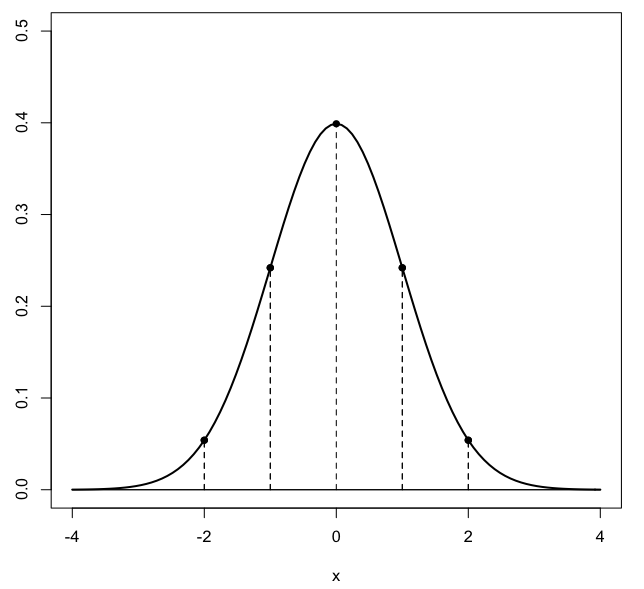
\includegraphics [scale=0.4] {gauss3.png} \end{center}
\begin{document}
\maketitle
\Large
Normally, books on complex analysis get into Laurent series and lots of theorems at this point.  However, I want to look ahead to Residue theory, which is really the reason for all the series stuff, then we'll spend some time with Taylor and Laurent.

\subsection*{Residues}
By definition the \emph{residue} at a simple pole $z_0$ is defined to be
\[ b_1 = \lim_{z \rightarrow z_0} (z-z_0) \ f(z)  \]
We get there from 
\[  \oint \frac{f(z)}{z - z_0} \ dz = 2 \pi i f(z_0) \]
Just think of it as in the limit that $z \rightarrow z_0$, the denominator $z-z_0$ on the left of the first equation is a constant, so we can multiply both sides by $z - z_0$
to obtain the result for the residue.
\[ \oint f(z) \ dz = 2 \pi i \ \lim_{z \rightarrow z_0} (z-z_0) \ f(z)  \]
using the definition
\[ b_1 = \lim_{z \rightarrow z_0} (z-z_0) \ f(z)  \]
we obtain
\[ \oint f(z) \ dz = 2 \pi i \ b_1  \]
If there is more than one such point
\[ \oint f(z) \ dz = 2 \pi i \ \sum \text{ Res } \]
The value of the integral is $2 \pi i$ times the sum of all the residues enclosed by the path.

\subsection*{residues}
We repeat the problem from last time, using residues.  
\[ \oint f(z) \ dz = \oint \frac{1}{z^2 + 1} \ dz \]

Our formula is:
\[ b_1 = \lim_{z \rightarrow z_0} (z-z_0) \ f(z)  \]
and
\[ \oint f(z) \ dz = 2 \pi i \ \sum \text{ Res } \]

Evaluate the first equation:
\[ b_1 = \lim_{z \rightarrow z_0} (z-z_0) \ f(z)  \]
\[ = \lim_{z \rightarrow i} (z-i) \  \frac{1}{(z+i)(z-i)} \]
\[ = \frac{1}{2i} \]
And by the second equation:
\[ I = \pi \]
as before.  Seems a bit easier!

If the unit circle had been centered at $-i$, rewrite the function as
\[ f(z) = \frac{1/z-i}{z+i} \]
The value of the function is
\[ \frac{1}{z-i}(-i) = -\frac{1}{2i} \]
and that integral is then $- \pi$.

A contour that includes both singularities integrates to zero.

\subsection*{example}
In this section we get more practice.

\[ \oint_C \frac{e^z}{z^2 - 2z - 3} \ dz \]
The denominator can be factored
\[ z^2 - 2z - 3 = (z + 1)(z - 3) \]
if our disk contains $|z \le 2|$ then it includes only $z = -1$ and our formula
\[ b_1 = \lim_{z \rightarrow z_0} (z-z_0) \ f(z)  \]
so
\[ b_1 = \lim_{z \rightarrow -1} (z+1) \ \frac{e^z}{(z + 1)(z - 3)}  \]
\[ = \lim_{z \rightarrow -1} \ \frac{e^z}{(z - 3)}  \]
\[ = \frac{e^{-1}}{-1 - 3} = - \frac{1}{4 e} \]
and
\[ I = 2 \pi i \ b_1 \]
\[ = 2 \pi i \ (- \frac{1}{4 e}) \]
\[ = - \frac{\pi i}{2 e} \]

\subsection*{example}
\[ \int \frac{5z-2}{z(z-1)} \ dz \]
There are two simple poles at $z_0 = 0$ and $z_0 = 1$ and the residues are
\[ \text{Res }(0) = \lim_{z \rightarrow 0} (z - 0) \ \frac{5z-2}{z(z-1)} \]
\[ = \lim_{z \rightarrow 0} \ \frac{5z-2}{(z-1)} \]
\[ = \frac{5 \cdot 0 - 2}{0 - 1} = 2 \]
\[ \text{Res }(1) = \lim_{z \rightarrow 1} (z - 1) \ \frac{5z-2}{z(z-1)} \]
\[ = \lim_{z \rightarrow 1} \ \frac{5z-2}{z} \]
\[ = \frac{5 \cdot 1 - 2}{1} = 3 \]
Hence the total of all the residues is $5$ and $I = 10 \pi i$.

\subsection*{example}
Consider
\[ \int \frac{1}{z^4 - 1} \ dz \]
We can factor the denominator as
\[ z^4 - 1 = (z^2 - 1)(z^2 + 1) \]
\[ = (z+1)(z-1)(z+i)(z-i) \]
We see that there are four poles, and each will have a residue.
\[ \text{Res}(1) =  \lim_{z \rightarrow 1} (z-1) \ \frac{1}{(z+1)(z-1)(z+i)(z-i)} \]
\[ =  \lim_{z \rightarrow 1} \ \frac{1}{(z+1)(z+i)(z-i)} \]
\[ = \frac{1}{2(1+1)} = \frac{1}{4} \]
\[ \text{Res}(i) =  \lim_{z \rightarrow i} (z-i) \ \frac{1}{(z+1)(z-1)(z+i)(z-i)} \]
\[ \text{Res}(i) =  \lim_{z \rightarrow i} \ \frac{1}{(z+1)(z-1)(z+i)} \]
\[ =  \lim_{z \rightarrow i} \ \frac{1}{(z^2 - 1)(z+i)} \]
\[ = \frac{1}{(-2)(2i)} = -\frac{1}{4i} = \frac{i}{4}  \]

\subsection*{Removable singularities}
If the residue turns out to be equal to zero, that is a removable singularity.  
\[ I = \int_C \frac{\sin \pi z}{z^2 - 1} \ dz \]
The denominator can be factored into 
\[ z^2 - 1 = (z + 1)(z - 1) \]
Suppose $C$ includes only $z = 1$, then
\[ \text{Res}(1) = \lim_{z \rightarrow 1}  (z-1) \ \frac{\sin \pi z}{(z + 1)(z - 1)} \]
\[ = \lim_{z \rightarrow 1} \ \frac{\sin \pi z}{(z + 1)} = \frac{\sin \pi}{2} =  0 \]

Here's a trick:
\[ f(z) = z^2 \sin \frac{1}{z} \]
Compute Res$(0)$
\[ \sin \frac{1}{z} = \frac{1}{z} - \frac{1}{3!} \ \frac{1}{z^3} + \frac{1}{5!} \ \frac{1}{z^5} \dots \]
\[ z^2 \sin \frac{1}{z} = z - \frac{1}{3!} \ \frac{1}{z} + \frac{1}{5!} \ \frac{1}{z^3} \dots \]
The only non-zero integral term is 
\[ - \frac{1}{3!} \ \frac{1}{z} \]
and the residue there is
\[ \lim_{z \rightarrow 0} \ (z - 0) (- \frac{1}{3!} \ \frac{1}{z}) \]
\[ = - \frac{1}{3!} = - \frac{1}{6} \]

\end{document}  
